%% Available online at https://www.overleaf.com/11445166drmnqzsywytj#/43230232/

\documentclass[11pt]{article}

\usepackage{booktabs}
\usepackage{homeworkpkg}
\usepackage{enumitem}
\usepackage[font=small,labelfont=bf]{caption}
\usepackage[bottom]{footmisc}
\usepackage{multicol}
\usepackage{multirow}
\usepackage[main=english,german]{babel}
\usepackage[T1]{fontenc}

\newlength\dunder
\settowidth{\dunder}{\_}

\graphicspath{ {images/} }

%% Local Macros and packages: add any of your own definitions here.

\begin{document}

% Homework number, your name and NetID, and optionally, the names/NetIDs of anyone you collaborated with. If you did not collaborate with anybody, leave the last parameter empty.
\homework
    {1}
    {Nestor Alejandro Bermudez Sarmiento (nab6)}
    {}

\section*{Introduction}
The following report discusses the result of using AutoPhrase and Word2Vec over two different data sets to find quality phrases and later on group them using unsupervised clustering methods.\\

The data sets in question are a sample of the DBLP and YELP data sets commonly used in data mining performance reports. \\

The code used to perform the experiments can be found on GitHub \footnote{\url{https://github.com/nbermudezs/UIUC_CS512/tree/master/assignment_1}}. Attached with this report you will find some of the results. These include the mined phrases (both single and multi words), the embeddings for the mined phrases and a file containing all the clusters and the corresponding phrases on each for each of the data sets.

\section*{Setup and Experiment Design}
The experiments were performed in a macOS system; word2vec was downloaded and compiled using C; the clustering code was written in Python and the code to automatically run all the different setups was written in Bash. All the original code can be found in my GitHub repo.\\

The experiments consisted of trying different values for both \textit{HIGHLIGHT\_MULTI} and \textit{HIGHLIGHT\_SINGLE}. Due to the time it takes to run each setting only 25 settings were performed on each data set. \\
For both variables the values tried were: 0.1, 0.3, 0.5, 0.7, 0.9.

\section*{Results}
This section includes some of the phrases found for each of the data sets, statistics about them and some examples of the clusters. \\

Lets first start by looking at some of the mined phrases for both single and multi word.

\subsection*{DBLP}
\subsubsection*{Top-30 phrases (multiple words)}
sun microsystems;
disaster relief;
authorship attribution;
vickrey auctions;
marching cubes;
liner shipping;
microsoft excel;
spanning trees;
turbo equalization;
spreading activation;
wind turbines;
brazilian portuguese;
bell labs;
homomorphic encryption;
google scholar;
simultaneous multithreading;
isabelle hol;
noun phrase;
multiset rewriting;
liquid crystal;
epipolar geometry;
blood glucose;
minimally invasive surgery;
colon cancer;
doctoral consortium;
convex hulls;
chip multiprocessors;
ssl tls;
sleep apnea;
river basin;

\subsubsection*{Top-30 phrases (single word)}
pearl;
lai;
lustre;
ajax;
inp;
estelle;
andrew;
allen;
mathematica;
tracer;
isis;
mbps;
vdd;
powerpoint;
yang;
xen;
finnish;
stern;
turkey;
cisco;
mason;
jim;
mosfets;
lin;
medline;
hu;
insar;
taiwanese;
promela;
sparc;

\subsubsection*{Middle-30 phrases (multiple words)}
binary moment;
von mr;
fundamental aspect;
synchronous data;
an important building block;
simulation of;
single data set;
explicit word;
obey certain;
2005 2006;
at different sites;
randomized distributed;
zero characteristic
marriage between;
systems for strategic;
scalability and dynamic;
systems for digital;
networking and applications;
applications on embedded;
applications and platforms;
dynamics in complex;
systems for industrial;
applications of geometric;
applications for small;
stability for systems;
computing in java;
systems for effective;
control and routing;
developed and combined;
techniques in reducing;

\subsubsection*{Middle-30 phrases (single word)}
preferences;
influencing;
jscc;
fre;
unobserved;
v2.0;
kommerzielle;
murmurs;
topaz;
imprints;
clavier;
troubleshooter;
pseudotriangulations;
dramaturgical;
separatrix;
prospection;
bubbly;
tree's;
spiculated;
misfolding;
conciliating;
lizard;
montages;
percolating;
condensate;
reputational;
elementwise;
illocutionary;
hunger;
muscl;

\subsubsection*{Bottom-30 phrases (multiple words)}
and effective approach to;
the theoretical limit of;
a standard database of;
the typical characteristics of;
a specific feature of;
an optimal selection of;
the asymptotic capacity of;
the basic mechanisms of;
a common interface to;
a fading channel with;
a program logic for;
a prior distribution on;
a fundamental change in;
this algorithm runs in;
the creation and manipulation of;
a requirements analysis for;
a necessity to;
an implementation model of;
the knowledge stored in;
to fault tolerance in;
the inherent uncertainty in;
for relevance feedback in;
the data gathered by;
a uniform approach for;
the underlying geometry of;
an estimation method of;
the total number of processors in;
the factors leading to;
the concepts presented in;
the topics discussed in;

\subsubsection*{Bottom-30 phrases (single word)}
βo;
cktsteiner;
fotw;
votc;
λ3;
pieceware;
udupa;
lpoll;
iszero;
changelog;
mkj;
blogreg;
pcvms;
glazier;
syncsql;
rpprimary;
pp2a;
ifml;
geeve;
qlab;
wgmww;
modc;
bcri;
cvwann;
pidis;
arwon;
sadr;
laac;
pcsw;
rfpf;


\subsection*{YELP}
\subsubsection*{Top-30 phrases (multiple words)}
noble beast;
tom's thumb;
papago park;
farmers market;
fox news;
jason's deli;
fettuccine alfredo;
golden corral;
xtreme bean;
eggs benedict;
britney spears;
pub crawl;
loco patron;
la canasta;
mason jar;
anchor steam;
fox concepts;
bon appetite;
gainey village;
palm springs;
ajo al's;
tammy coe;
pollo fundido;
daily dose;
brussels sprouts;
hobby lobby;
barrio queen;
coney island;
frank sinatra;
blue moon;
\subsubsection*{Top-30 phrases (single word)}
redbox;
coach;
ale;
mormon;
samurai;
hef;
serrano;
raspberry;
police;
antipasto;
yelper;
naan;
lululemon;
smith;
northern;
chimichanga;
mimosa;
sochu;
latin;
ristorante;
mocha;
sichuan;
meatloaf;
philly;
magazine;
sirloin;
fridays;
fondue;
panini;
mole;
\subsubsection*{Middle-30 phrases (multiple words)}
the feta;
a bad seat;
not so nice;
2 x;
for mother's day;
more than one star;
a quick serve;
a drug store;
planned on getting;
this aj's;
a video game;
haven't already;
a bit doughy;
bf liked;
you'll ever taste;
a much needed;
yelp about;
very chill;
increase in;
at bobby q;
mind paying more for;
sucker for;
a bit snooty;
a topping;
we'll definitely go back;
no option;
to solve;
3 to 4 stars;
a loooong;
a trailer;
\subsubsection*{Middle-30 phrases (single word)}
td;
ots;
aimlessly;
growlers;
za'atar;
collector;
milder;
committed;
backside;
resulting;
granita;
frequency;
indulging;
panel;
grrrrr;
distant;
sprung;
yasha;
schwag;
tracker;
ravs;
locating;
mahogany;
puzzled;
customer;
raffle;
lps;
fellas;
cubes;
scrambled;
\subsubsection*{Bottom-30 phrases (multiple words)}
a great place to come with;
even longer for;
want to stop in;
any place i've;
get busy but;
five minutes to get;
to bring back to;
and it's easy to;
to play with and;
a little small and;
little patio with;
so long to go;
so easy to get;
a little extra to;
the staff does not;
to agree to;
to head back and;
to feel like you're;
not always easy to;
to live here;
so cool to;
the manager came by to;
it's amazing to;
really really wanted to;
take long to get;
a perfectly made;
no reason to go to;
any other place in;
this location for about;
to go inside to;
\subsubsection*{Bottom-30 phrases (single word)}
were;
be;
was;
is;
are;
could;
has;
have;
been;
itself;
can;
ourselves;
which;
gives;
your;
had;
would;
should;
ought;
him;
causes;
merely;
containing;
werent;
am;
them;
arent;
|;
might;
07;


\subsection*{Statistics}
For each of the settings of the experiment, the number of phrases segmented and the average number of phrases on each sentence was capture. The results in the following table show the metrics for the recommended setting (HIGHLIGHT\_MULTI = \textbf{0.5}, HIGHLIGHT\_SINGLE=\textbf{0.9}).\\
\begin{center}
	\begin{tabular}{r|r|r|l}
	\cline{2-3}
	& \multicolumn{2}{ c| }{Data set} \\ \cline{2-3}
	& DBLP & YELP \\ \cline{1-3}
	
	\multicolumn{1}{ |l| }{\# Phrases} & 7,877,383 & 1,587,940 \\ \cline{1-3}
	\multicolumn{1}{ |l| }{Avg. Phrases/Sentence} & 0.597369 & 0.38297 \\ \cline{1-3}
	\end{tabular}
	\captionof{table}{Number of phrases and average per sentence.}
\end{center}

\pagebreak

\subsection*{Clusters}
Although multiple clustering methods exist, DBSCAN, $k$-Means, AGNES, I decided to use spherical $k$-Means, which is nothing more than the regular $k$-Means using \textbf{cosine} as the distance measure. Experiments were performed using 10, 20, 40 and 80 cluster centers. For the sake of pragmatism only the phrases selected from the clustering with 40 centers are shown in this report but everything else can be found in the GitHub, including best effort labels for some of the clusters. Some interesting finds will be discussed in this section.

\subsubsection*{DBLP}
\textbf{Cluster 29 (Databases/Data Mining)}:
\begin{multicols}{3}
POS Tagging\\
Frequent Pattern Mining\\
Text Corpora\\
Heterogeneous Data\\
Sequential Pattern Mining\\
Knowledge Extraction\\
Data Preparation\\
Information Extraction\\
Feature Mining\\
Spatio-Temporal Data\\
Graph Structure\\
Biological Networks\\
Database Theory\\
Data Clustering\\
Sequence Database\\
Semi-Structured Data\\
Image Retrieval Systems\\
Database Views\\
Mining Algorithms\\
Bitemporal Databases
\end{multicols}

\textbf{Cluster 15 (German words)}:
\begin{multicols}{3}
Qualität der\\
Künstliche Intelligenz\\
Diagramas de\\
Techniken und\\
Zur Theorie der\\
Ansätze für\\
Modell und\\
Ein objektorientierter\\
Die Programmiersprache\\
Bedeutung von\\
Und Semantik\\
Eine Herausforderung\\
Des Wissensmanagements\\
Integrierter Ansatz\\
Neue Herausforderungen\\
Zur Erfassung\\
Netze mit\\
Kosten und\\
Nach der\\
Erste Erfahrungen
\end{multicols}

\textbf{Cluster 17 (Networks)}:
\begin{multicols}{3}
Wi-Fi\\
TCP/IP\\
Ad hoc networks\\
Packet level\\
Low bandwidth\\
Congestion control\\
ATM networks\\
Real-time traffic\\
QoS provisioning\\
Multicast protocols\\
Local area networks\\
IP traffic\\
Packet routing\\
Distributed Hash Tables\\
QoS guarantees\\
TCP-based\\
WiMAX-networks\\
Optimal routing\\
WPANs\\
3G networks
\end{multicols}

\textbf{Cluster 23 (Embedded Systems)}:
\begin{multicols}{3}
FPGA-based\\
Multi-core\\
Embedded system\\
Floating-point\\
Low latency\\
GPU-based\\
AMD\\
Cache memory\\
File access\\
Bus-based\\
Dual-core\\
High Performance Computing\\
Hardware Architectures\\
Read-write\\
NoC-based\\
Multi-core architectures\\
FPGA-technology\\
NAND flash\\
Per cycle\\
Block transfer
\end{multicols}

\textbf{Cluster 34 (Artificial Intelligence)}:
\begin{multicols}{3}
Support vector machines\\
Binary classification\\
Semi-supervised learning\\
Statistical inference\\
Parameter selection\\
EM algorithm\\
Kernel regression\\
Random Forest\\
Graphical model\\
LDA-based\\
Gradient ascent\\
Q-learning\\
Kernel PCA\\
Bayesian network classifiers\\
Naive Bayes\\
Markov networks\\
Backpropagation algorithm\\
Neural nets\\
Risk minimization\\
Score function
\end{multicols}

\subsubsection*{YELP}
\textbf{Cluster 10 (Deserts/Sweets)}:
\begin{multicols}{3}
Cake\\
Espresso\\
Cupcake\\
Whipped cream\\
Brownie\\
Pumpkin\\
Sundae\\
Pecan pie\\
Indulgence\\
Pound cake\\
Shake\\
Cinnamon rolls\\
Oreo\\
Buttercream frosting\\
Peanut butter cup\\
Custard\\
Flavored ice cream\\
Chocolate caramel\\
Ghirardelli\\
Coconut sorbet
\end{multicols}

\textbf{Cluster 24 (Point of Interest Names)}:
\begin{multicols}{3}
Walgreens\\
FroYo\\
Subway\\
Safeway\\
Denny's\\
Costco\\
Target\\
Total Wine\\
Pizza Hut\\
Chinese restaurants\\
Wal-Mart\\
Starbucks\\
Sprouts\\
Wildflower Bread\\
Sushi Roku\\
Mc Donalds\\
MoJo\\
Souper Salad\\
Farm Grill\\
TJ Maxx
\end{multicols}

\textbf{Cluster 28 (Traffic/Vehicle related)}:
\begin{multicols}{3}
Shuttle service\\
Monorail\\
Circle K\\
Ride bikes\\
Park area\\
Terminal to terminal\\
Honda Civic\\
Rental cars\\
Ducati\\
Parking lot\\
Stree parking\\
Garage\\
24/7\\
Boarding passes\\
Neon sign\\
High traffic\\
Light speed\\
Break room\\
Rail line\\
Passers by
\end{multicols}

\pagebreak

\textbf{Cluster 29 (Drinks)}:
\begin{multicols}{3}
Margarita\\
Iced tea\\
Sangria\\
Guinness\\
Martini\\
Gin\\
Draft beer\\
Ale\\
Shot glass\\
Pinot Grigio\\
Red Bull\\
Stella\\
Jamaica\\
Drip coffee\\
Vodka soda\\
Cuervo\\
Pint glass\\
Oolong\\
24 oz\\
Ladies Night
\end{multicols}

\textbf{Cluster 39 (Service/Staff/QoS)}:
\begin{multicols}{3}
Super nice\\
Great customer service\\
Hostess\\
Cashier\\
Extremely friendly\\
Table service\\
Kid friendly\\
Barista\\
Speak English\\
Customer service\\
Freaking awesome\\
Big smiles\\
Extremely knowledgable\\
Service sucks\\
Fitting room\\
Great instructors\\
Service provider\\
Cute waiter\\
Wine guy\\
Personalized service
\end{multicols}

\textbf{Cluster 33 (Payment and Prices)}:
\begin{multicols}{3}
Free\\
Discount\\
\$1.50\\
Totally worth\\
Unlimited\\
Bonus\\
Triple\\
\$5.50\\
\$9.99\\
Price tag\\
Ten dollars\\
Resort fee\\
Admission\\
\$50.00\\
\$5.25\\
Tip\\
lb\\
18\% gratuity\\
Automatically added\\
Half price
\end{multicols}

\subsubsection*{Comparison}
As mentioned before, the clustering was done using 10, 20, 40 and 80 centers. It was particularly interesting to see how the granularity of some of the groups increased as the number of centers increased.\\

For example, for the DBLP data set, when using 10 centers one of them had phrases that could be categorized as "CS Theory" which include things like algorithms, optimization, discrete math; after using 20 centers it was possible to find smaller clusters that were more "specialized", there were clusters that could be identified as "CS Theory | Graphs", "CS Theory | Algorithms", "CS Theory | Optimization". \\

Some specific examples: \\
\textbf{CS Theory | Optimization}: non-stationary, cost functions, objective functions, probability distributions, covariance matrix, least squares, design problem, Markov chain, confidence interval, stochastic processes.\\
\textbf{CS Theory | Graphs}: point sets, planar graphs, shortest path, random graph, directed graphs, spanning trees, matching problem, Nash equilibrium, Voronoi diagram.\\
\textbf{CS Theory | Algorithms}: SAT solver, well behaved, formally proved, Von Neuman, PSPACE-complete, theorem provers, canonical form, mathematical models, PL/I, Allen, formally verified.\\

A similar situation was found for the YELP data set. When using 10 centers there was only one cluster that included phrases that identified "Points of Interest", when using 40 centers at least 3 clusters had POIs in it. Unfortunately I was not able to find a pattern to discern what the difference between those 3 clusters were.\\

The full data, including some named clusters for each number of centers can be found the GitHub repo.

\subsection*{Parameter analysis}
Finally lets look at how the number of segmented phrases and the average number of phrases per sentence changes as the parameters of the segmentation script change. As mentioned earlier in this report 5 values were tried for each of the highlight thresholds resulting in 25 settings. The following plots represent the changes on both metrics as one of the variables changes while keeping the second fixed.

\subsubsection*{DBLP}
\begin{multicols}{2}
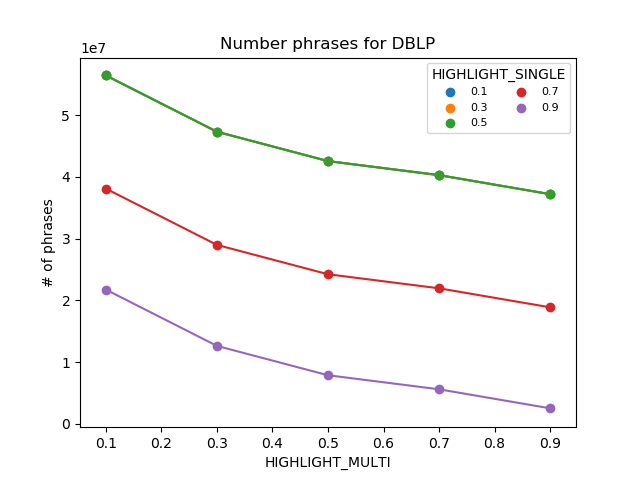
\includegraphics[scale=0.27]{n_phrases_dblp.png}

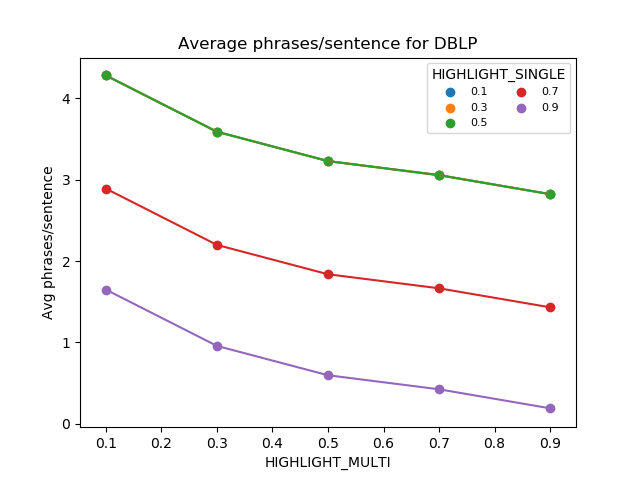
\includegraphics[scale=0.27]{avg_phrases_dblp.png}
\end{multicols}


\subsubsection*{YELP}
\begin{multicols}{2}
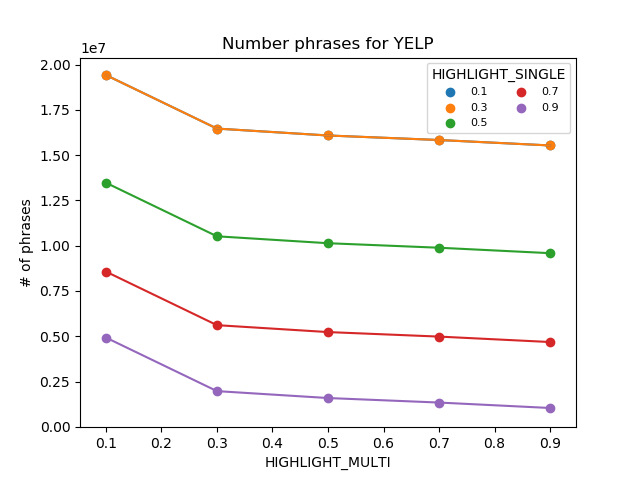
\includegraphics[scale=0.27]{n_phrases_yelp.png}

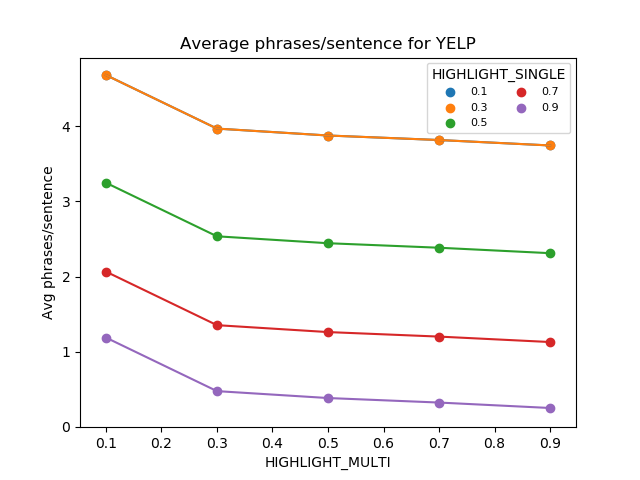
\includegraphics[scale=0.27]{avg_phrases_yelp.png}
\end{multicols}


\end{document}